\chapter{Sequential Circuits}
\graphicspath{ {./chapter05/FigWork} }
%%%%%%%%%%%%%%%%%%%%%%%%%%%%%%%%%%%%%%%%%%%%%%%%%%%%
%% Here are the helpfull stuff
%%%%%%%%%%%%%%%%%%%%%%%%%%%%%%%%%%%%%%%%%%%%%%%%%%%%
\section{Helpful Stuff}

\textit{ When} the bit is stored.
\begin{enumerate}
	\item Latches - a latch continuously samples its inputs.  Latches do not have
	a clock input.
	\item Clocked latches - a clocked latch samples its inputs when the clock input equals 1.
	When the clock input equals 0 the clocked latch does not change the currently stored bit.
	\item Flip flops - a flip flop samples its input when the its clock input rises.  The
	clock is said to rise when it goes from a logic 0 to a logic 1.
	When the clock input is not rising the flip flop does not change the currently stored bit.
\end{enumerate}
\textit{ How} the input(s) is transformed into a stored bit.


\begin{tabular}{p{2in}p{2in}}

\begin{tabular}{l||l}
D & Q+   \\ \hline
0 & 0 \\ \hline
1 & 1 \\
\end{tabular}

\vspace{0.2in}
&
\begin{tabular}{c||c}
T & Q+   \\ \hline
0 & Q \\ \hline
1 & Q' \\
\end{tabular} 
\vspace{0.2in} \\

\begin{tabular}{c|c||c}
S & R & Q+   \\ \hline
0 & 0 & Q \\ \hline
0 & 1 & 0 \\ \hline
1 & 0 & 1 \\ \hline
1 & 1 & x \\
\end{tabular}
&
\begin{tabular}{c|c||c}
J & K & Q+   \\ \hline
0 & 0 & Q \\ \hline
0 & 1 & 0 \\ \hline
1 & 0 & 1 \\ \hline
1 & 1 & Q' \\
\end{tabular} \\

\end{tabular}

\vspace{0.2in}

The \textit{ When} and \textit{ How} dimensions are arranged in the
following table.

\begin{tabular}{|c|c|c|c|}\hline
   &  Latch & Clocked Latch  & Flip Flop   \\ \hline
D  &        &	&	\\ \hline
T  &        &     &	\\ \hline
SR &	    	&	&	\\ \hline
JK &        &     &	\\ \hline
\end{tabular}


%%%%%%%%%%%%%%%%%%%%%%%%%%%%%%%%%%%%%%%%%%%%%%%%%%%%
%% Here are terms that the students define
%%%%%%%%%%%%%%%%%%%%%%%%%%%%%%%%%%%%%%%%%%%%%%%%%%%%



%%%%%%%%%%%%%%%%%%%%%%%%%%%%%%%%%%%%%%%%%%%%%%%%%%%%
%% Here are the problems
%%%%%%%%%%%%%%%%%%%%%%%%%%%%%%%%%%%%%%%%%%%%%%%%%%%%
\pagebreak
\section{Problems}
Here are some problems to work on.
\begin{description}
\item[Complete the state table with the help of the following figures.]

\begin{tabular}{c|c||c|c}
S & R & Q$^+$ & Q$'^+$ \\ \hline
0 & 0 &  &  \\ \hline
0 & 1 &  &  \\ \hline
1 & 0 &  &  \\ \hline
1 & 1 &  &  \\
\end{tabular}

\begin{tabular}{p{2in} p{2in}}
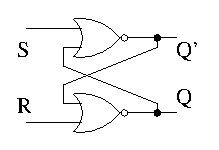
\includegraphics{SRlatch} & 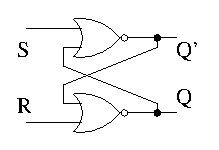
\includegraphics{SRlatch} \\ 
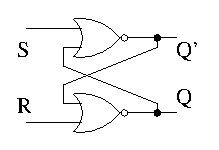
\includegraphics{SRlatch} & 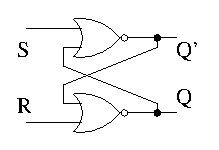
\includegraphics{SRlatch} \\
\end{tabular}

\vspace{0.2in} 

\item[Complete the timing diagram.]

\scalebox{0.5}{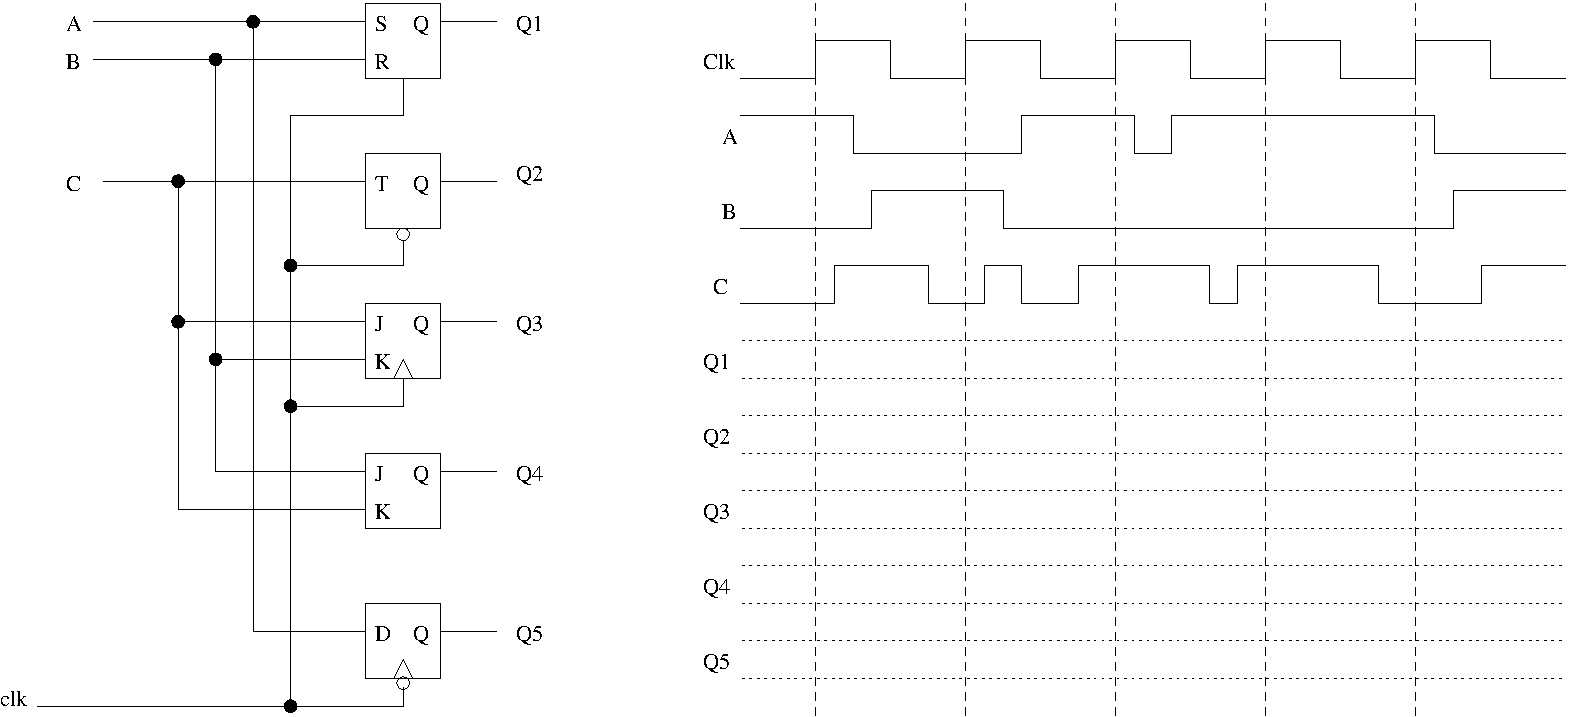
\includegraphics{BMEtime}}
\end{description}

